\chapter{Dosažené výsledky}
V této kapitole se budeme zabývat měřením konkrétních vzorků, interpretací spekter a porovníní výsledů obou užitých metod. U obou použitých 
metod měříme v polární geometrii, přičemž dopad na vzrorek je téměř kolmý. Magnetické pole generované magnetem je u modulační metody 1.2 T. Magnet 
použitý při metodě zkřížených polarizátorů generuje pouze 0.4 T.

\section{Ultratenké vrstvy La$_{2/3}$Sr$_{1/3}$MnO$_3$}
První sada zkoumaných vzorků jsou tenké vrstvy La$_{2/3}$Sr$_{1/3}$MnO$_3$ (LSMO). Tento materiál je zkoumán předevšm kvůli jeko potenciálnímu použití v oblasti spintroniky. 
Ta vyžaduje, aby materiál měl různou vodivost pro různě spiny elektronů. Další důležitý požadavek je jejich Curiova teplota alespoň nad pokojovou teplotou, z důvodu 
použitelnosti v zařízeních pracujících právě při pokojové teplotě.

Tyto vzorky byly vyrobeny metodou pulsní laserové depozice (PLD). Tato metoda umožňuje vytváření tenkých filmů o tloušťkách menších než 50 nm. Ve zkratce metoda funguje na principu kondenzace plasmy odpařované za pomoci krátkých laserových pulsů. 
Tyto vzorky byly připraveny na substrátu SrTiO$_3$ (STO) s krystalografickou orientací (1 0 0) 
a mřížkovou konstantou $a_{STO}=3.905$ \AA. Mřížková konstanta LSMO je $a_{LSMO}=3.889$ \AA, důsledkem čehož dochází k pnutí v tenké vrtvě, což má za následek slabší feromagnetické vlastnosti. 
Tloušťky zkoumaných vzorků byly 23,1 nm (PLD 186) a 80,8 nm (PLD202). 

Výsledky měření těchto vzorků jsou na obrázcích (\ref{sPLD186}) a (\ref{sPLD202}).
Na spektrech je vidět, že modulační metoda 
dává pro energie nad 4.3 eV nepřesné výsledky. V této oblasti je vidět pokles obou ekeftů k nule, 
který je způsoben postupnou ztrátou signálu na detektoru. Tu má na vině 
snížení účinnosti fotonásobiče, která by mohla být odstraněna například použitím fotonásobiče s obálkou z křemenného skla, které má výrazně lepší propustnost v UV.

Dále je znatelný posun celého spekra. To je následek horšího spektrálního rozlišení monochromátoru. K tomu se ještě projevuje chybovost krokového motorku, který 
způsobuje další nepřesnost v určení vlnové délky světla.

Až na výše uvedené vady je vidět velmi dobrá shoda spekter obou metod. Díky tomu můžeme říct, že metoda zkřížených polarizátorů má stejně, jako modulční metoda, velmi 
vysokou citlivost.

Ze vztahu (\ref{teor kerr}) můžme určit teoretické spektrum těchto vzorků. Hodnoty pro LSMO byli určeny na 35 nm tenké vrstvě, která 
se již dá považovat za téměř objemový materiál.  Parametry STO pak byly získány za pomoci elipsometrie. Výsledné porovnání 
teoretických hodnot s výsledky metody zkřížených polarizátorů obou 
vzorků je zobrazeno na obrázcích (\ref{sPLD186t}) a (\ref{sPLD202t}). Vidíme, že pro PLD186 jsme, až na velikost amplitudy, získaly totožné hodnoty. 
Tento rozdíl je dán tím, že materiálové konstanty byly určeny za nižší teploty. Díky shodě s teorií můžeme říct, že vzorek PLD186 má objemové vlastnosti LSMO. 
U vzorku PLD202 již vidíme, že ke shodě nedošlo. Z toho vyplývá, že muselo dojít ke změně krystalografické struktury, která vedla ke změně magnetooptických vlastností.

\begin{figure}
% GNUPLOT: LaTeX picture with Postscript
\begingroup
  \makeatletter
  \providecommand\color[2][]{%
    \GenericError{(gnuplot) \space\space\space\@spaces}{%
      Package color not loaded in conjunction with
      terminal option `colourtext'%
    }{See the gnuplot documentation for explanation.%
    }{Either use 'blacktext' in gnuplot or load the package
      color.sty in LaTeX.}%
    \renewcommand\color[2][]{}%
  }%
  \providecommand\includegraphics[2][]{%
    \GenericError{(gnuplot) \space\space\space\@spaces}{%
      Package graphicx or graphics not loaded%
    }{See the gnuplot documentation for explanation.%
    }{The gnuplot epslatex terminal needs graphicx.sty or graphics.sty.}%
    \renewcommand\includegraphics[2][]{}%
  }%
  \providecommand\rotatebox[2]{#2}%
  \@ifundefined{ifGPcolor}{%
    \newif\ifGPcolor
    \GPcolorfalse
  }{}%
  \@ifundefined{ifGPblacktext}{%
    \newif\ifGPblacktext
    \GPblacktexttrue
  }{}%
  % define a \g@addto@macro without @ in the name:
  \let\gplgaddtomacro\g@addto@macro
  % define empty templates for all commands taking text:
  \gdef\gplbacktext{}%
  \gdef\gplfronttext{}%
  \makeatother
  \ifGPblacktext
    % no textcolor at all
    \def\colorrgb#1{}%
    \def\colorgray#1{}%
  \else
    % gray or color?
    \ifGPcolor
      \def\colorrgb#1{\color[rgb]{#1}}%
      \def\colorgray#1{\color[gray]{#1}}%
      \expandafter\def\csname LTw\endcsname{\color{white}}%
      \expandafter\def\csname LTb\endcsname{\color{black}}%
      \expandafter\def\csname LTa\endcsname{\color{black}}%
      \expandafter\def\csname LT0\endcsname{\color[rgb]{1,0,0}}%
      \expandafter\def\csname LT1\endcsname{\color[rgb]{0,1,0}}%
      \expandafter\def\csname LT2\endcsname{\color[rgb]{0,0,1}}%
      \expandafter\def\csname LT3\endcsname{\color[rgb]{1,0,1}}%
      \expandafter\def\csname LT4\endcsname{\color[rgb]{0,1,1}}%
      \expandafter\def\csname LT5\endcsname{\color[rgb]{1,1,0}}%
      \expandafter\def\csname LT6\endcsname{\color[rgb]{0,0,0}}%
      \expandafter\def\csname LT7\endcsname{\color[rgb]{1,0.3,0}}%
      \expandafter\def\csname LT8\endcsname{\color[rgb]{0.5,0.5,0.5}}%
    \else
      % gray
      \def\colorrgb#1{\color{black}}%
      \def\colorgray#1{\color[gray]{#1}}%
      \expandafter\def\csname LTw\endcsname{\color{white}}%
      \expandafter\def\csname LTb\endcsname{\color{black}}%
      \expandafter\def\csname LTa\endcsname{\color{black}}%
      \expandafter\def\csname LT0\endcsname{\color{black}}%
      \expandafter\def\csname LT1\endcsname{\color{black}}%
      \expandafter\def\csname LT2\endcsname{\color{black}}%
      \expandafter\def\csname LT3\endcsname{\color{black}}%
      \expandafter\def\csname LT4\endcsname{\color{black}}%
      \expandafter\def\csname LT5\endcsname{\color{black}}%
      \expandafter\def\csname LT6\endcsname{\color{black}}%
      \expandafter\def\csname LT7\endcsname{\color{black}}%
      \expandafter\def\csname LT8\endcsname{\color{black}}%
    \fi
  \fi
  \setlength{\unitlength}{0.0500bp}%
  \begin{picture}(7200.00,5040.00)%
    \gplgaddtomacro\gplbacktext{%
      \csname LTb\endcsname%
      \put(1210,704){\makebox(0,0)[r]{\strut{}-0.2}}%
      \put(1210,1213){\makebox(0,0)[r]{\strut{}-0.15}}%
      \put(1210,1722){\makebox(0,0)[r]{\strut{}-0.1}}%
      \put(1210,2231){\makebox(0,0)[r]{\strut{}-0.05}}%
      \put(1210,2739){\makebox(0,0)[r]{\strut{} 0}}%
      \put(1210,3248){\makebox(0,0)[r]{\strut{} 0.05}}%
      \put(1210,3757){\makebox(0,0)[r]{\strut{} 0.1}}%
      \put(1210,4266){\makebox(0,0)[r]{\strut{} 0.15}}%
      \put(1210,4775){\makebox(0,0)[r]{\strut{} 0.2}}%
      \put(1496,484){\makebox(0,0){\strut{} 1.5}}%
      \put(2263,484){\makebox(0,0){\strut{} 2}}%
      \put(3031,484){\makebox(0,0){\strut{} 2.5}}%
      \put(3798,484){\makebox(0,0){\strut{} 3}}%
      \put(4566,484){\makebox(0,0){\strut{} 3.5}}%
      \put(5334,484){\makebox(0,0){\strut{} 4}}%
      \put(6101,484){\makebox(0,0){\strut{} 4.5}}%
      \put(6869,484){\makebox(0,0){\strut{} 5}}%
      \put(308,2739){\rotatebox{-270}{\makebox(0,0){\strut{}Polární Kerrův jev [deg.]}}}%
      \put(4105,154){\makebox(0,0){\strut{}$E$/eV}}%
    }%
    \gplgaddtomacro\gplfronttext{%
      \csname LTb\endcsname%
      \put(5882,4602){\makebox(0,0)[r]{\strut{}$\theta^1_K$}}%
      \csname LTb\endcsname%
      \put(5882,4382){\makebox(0,0)[r]{\strut{}$\epsilon^1_K$}}%
      \csname LTb\endcsname%
      \put(5882,4162){\makebox(0,0)[r]{\strut{}$\theta^2_K$}}%
      \csname LTb\endcsname%
      \put(5882,3942){\makebox(0,0)[r]{\strut{}$\epsilon^2_K$}}%
    }%
    \gplbacktext
    \put(0,0){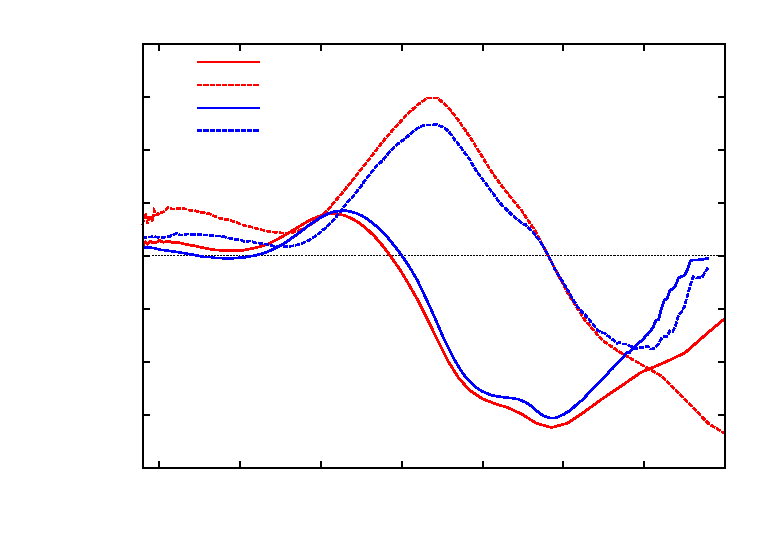
\includegraphics{grafy/PLD186}}%
    \gplfronttext
  \end{picture}%
\endgroup

\caption{Spektrum polárního Kerrova jevu vzorku PLD186. Červené křivky odpovídají metodě zkřížených polarizátorl, modré pak modulační metodě.}
\label{sPLD186}
\end{figure}

\begin{figure}
% GNUPLOT: LaTeX picture with Postscript
\begingroup
  \makeatletter
  \providecommand\color[2][]{%
    \GenericError{(gnuplot) \space\space\space\@spaces}{%
      Package color not loaded in conjunction with
      terminal option `colourtext'%
    }{See the gnuplot documentation for explanation.%
    }{Either use 'blacktext' in gnuplot or load the package
      color.sty in LaTeX.}%
    \renewcommand\color[2][]{}%
  }%
  \providecommand\includegraphics[2][]{%
    \GenericError{(gnuplot) \space\space\space\@spaces}{%
      Package graphicx or graphics not loaded%
    }{See the gnuplot documentation for explanation.%
    }{The gnuplot epslatex terminal needs graphicx.sty or graphics.sty.}%
    \renewcommand\includegraphics[2][]{}%
  }%
  \providecommand\rotatebox[2]{#2}%
  \@ifundefined{ifGPcolor}{%
    \newif\ifGPcolor
    \GPcolorfalse
  }{}%
  \@ifundefined{ifGPblacktext}{%
    \newif\ifGPblacktext
    \GPblacktexttrue
  }{}%
  % define a \g@addto@macro without @ in the name:
  \let\gplgaddtomacro\g@addto@macro
  % define empty templates for all commands taking text:
  \gdef\gplbacktext{}%
  \gdef\gplfronttext{}%
  \makeatother
  \ifGPblacktext
    % no textcolor at all
    \def\colorrgb#1{}%
    \def\colorgray#1{}%
  \else
    % gray or color?
    \ifGPcolor
      \def\colorrgb#1{\color[rgb]{#1}}%
      \def\colorgray#1{\color[gray]{#1}}%
      \expandafter\def\csname LTw\endcsname{\color{white}}%
      \expandafter\def\csname LTb\endcsname{\color{black}}%
      \expandafter\def\csname LTa\endcsname{\color{black}}%
      \expandafter\def\csname LT0\endcsname{\color[rgb]{1,0,0}}%
      \expandafter\def\csname LT1\endcsname{\color[rgb]{0,1,0}}%
      \expandafter\def\csname LT2\endcsname{\color[rgb]{0,0,1}}%
      \expandafter\def\csname LT3\endcsname{\color[rgb]{1,0,1}}%
      \expandafter\def\csname LT4\endcsname{\color[rgb]{0,1,1}}%
      \expandafter\def\csname LT5\endcsname{\color[rgb]{1,1,0}}%
      \expandafter\def\csname LT6\endcsname{\color[rgb]{0,0,0}}%
      \expandafter\def\csname LT7\endcsname{\color[rgb]{1,0.3,0}}%
      \expandafter\def\csname LT8\endcsname{\color[rgb]{0.5,0.5,0.5}}%
    \else
      % gray
      \def\colorrgb#1{\color{black}}%
      \def\colorgray#1{\color[gray]{#1}}%
      \expandafter\def\csname LTw\endcsname{\color{white}}%
      \expandafter\def\csname LTb\endcsname{\color{black}}%
      \expandafter\def\csname LTa\endcsname{\color{black}}%
      \expandafter\def\csname LT0\endcsname{\color{black}}%
      \expandafter\def\csname LT1\endcsname{\color{black}}%
      \expandafter\def\csname LT2\endcsname{\color{black}}%
      \expandafter\def\csname LT3\endcsname{\color{black}}%
      \expandafter\def\csname LT4\endcsname{\color{black}}%
      \expandafter\def\csname LT5\endcsname{\color{black}}%
      \expandafter\def\csname LT6\endcsname{\color{black}}%
      \expandafter\def\csname LT7\endcsname{\color{black}}%
      \expandafter\def\csname LT8\endcsname{\color{black}}%
    \fi
  \fi
  \setlength{\unitlength}{0.0500bp}%
  \begin{picture}(7200.00,5040.00)%
    \gplgaddtomacro\gplbacktext{%
      \csname LTb\endcsname%
      \put(990,704){\makebox(0,0)[r]{\strut{}-0.2}}%
      \put(990,1213){\makebox(0,0)[r]{\strut{}-0.15}}%
      \put(990,1722){\makebox(0,0)[r]{\strut{}-0.1}}%
      \put(990,2231){\makebox(0,0)[r]{\strut{}-0.05}}%
      \put(990,2739){\makebox(0,0)[r]{\strut{} 0}}%
      \put(990,3248){\makebox(0,0)[r]{\strut{} 0.05}}%
      \put(990,3757){\makebox(0,0)[r]{\strut{} 0.1}}%
      \put(990,4266){\makebox(0,0)[r]{\strut{} 0.15}}%
      \put(990,4775){\makebox(0,0)[r]{\strut{} 0.2}}%
      \put(1282,484){\makebox(0,0){\strut{} 1.5}}%
      \put(2080,484){\makebox(0,0){\strut{} 2}}%
      \put(2878,484){\makebox(0,0){\strut{} 2.5}}%
      \put(3676,484){\makebox(0,0){\strut{} 3}}%
      \put(4474,484){\makebox(0,0){\strut{} 3.5}}%
      \put(5273,484){\makebox(0,0){\strut{} 4}}%
      \put(6071,484){\makebox(0,0){\strut{} 4.5}}%
      \put(6869,484){\makebox(0,0){\strut{} 5}}%
      \put(308,2739){\rotatebox{-270}{\makebox(0,0){\strut{}}}}%
      \put(3995,154){\makebox(0,0){\strut{}$E$/eV}}%
    }%
    \gplgaddtomacro\gplfronttext{%
      \csname LTb\endcsname%
      \put(3102,4602){\makebox(0,0)[r]{\strut{}$\theta^1_K$}}%
      \csname LTb\endcsname%
      \put(3102,4382){\makebox(0,0)[r]{\strut{}$\epsilon^1_K$}}%
    }%
    \gplbacktext
    \put(0,0){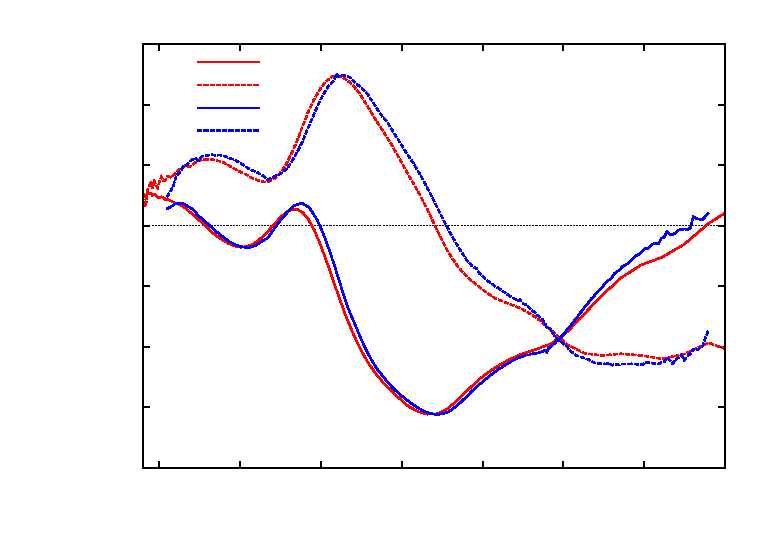
\includegraphics{PLD202}}%
    \gplfronttext
  \end{picture}%
\endgroup

\caption{Spektrum polárního Kerrova jevu vzorku PLD202. Červené křivky odpovídají metodě zkřížených polarizátorl, modré pak modulační metodě.}
\label{sPLD202}
\end{figure}

\begin{figure}
% GNUPLOT: LaTeX picture with Postscript
\begingroup
  \makeatletter
  \providecommand\color[2][]{%
    \GenericError{(gnuplot) \space\space\space\@spaces}{%
      Package color not loaded in conjunction with
      terminal option `colourtext'%
    }{See the gnuplot documentation for explanation.%
    }{Either use 'blacktext' in gnuplot or load the package
      color.sty in LaTeX.}%
    \renewcommand\color[2][]{}%
  }%
  \providecommand\includegraphics[2][]{%
    \GenericError{(gnuplot) \space\space\space\@spaces}{%
      Package graphicx or graphics not loaded%
    }{See the gnuplot documentation for explanation.%
    }{The gnuplot epslatex terminal needs graphicx.sty or graphics.sty.}%
    \renewcommand\includegraphics[2][]{}%
  }%
  \providecommand\rotatebox[2]{#2}%
  \@ifundefined{ifGPcolor}{%
    \newif\ifGPcolor
    \GPcolortrue
  }{}%
  \@ifundefined{ifGPblacktext}{%
    \newif\ifGPblacktext
    \GPblacktexttrue
  }{}%
  % define a \g@addto@macro without @ in the name:
  \let\gplgaddtomacro\g@addto@macro
  % define empty templates for all commands taking text:
  \gdef\gplbacktext{}%
  \gdef\gplfronttext{}%
  \makeatother
  \ifGPblacktext
    % no textcolor at all
    \def\colorrgb#1{}%
    \def\colorgray#1{}%
  \else
    % gray or color?
    \ifGPcolor
      \def\colorrgb#1{\color[rgb]{#1}}%
      \def\colorgray#1{\color[gray]{#1}}%
      \expandafter\def\csname LTw\endcsname{\color{white}}%
      \expandafter\def\csname LTb\endcsname{\color{black}}%
      \expandafter\def\csname LTa\endcsname{\color{black}}%
      \expandafter\def\csname LT0\endcsname{\color[rgb]{1,0,0}}%
      \expandafter\def\csname LT1\endcsname{\color[rgb]{0,1,0}}%
      \expandafter\def\csname LT2\endcsname{\color[rgb]{0,0,1}}%
      \expandafter\def\csname LT3\endcsname{\color[rgb]{1,0,1}}%
      \expandafter\def\csname LT4\endcsname{\color[rgb]{0,1,1}}%
      \expandafter\def\csname LT5\endcsname{\color[rgb]{1,1,0}}%
      \expandafter\def\csname LT6\endcsname{\color[rgb]{0,0,0}}%
      \expandafter\def\csname LT7\endcsname{\color[rgb]{1,0.3,0}}%
      \expandafter\def\csname LT8\endcsname{\color[rgb]{0.5,0.5,0.5}}%
    \else
      % gray
      \def\colorrgb#1{\color{black}}%
      \def\colorgray#1{\color[gray]{#1}}%
      \expandafter\def\csname LTw\endcsname{\color{white}}%
      \expandafter\def\csname LTb\endcsname{\color{black}}%
      \expandafter\def\csname LTa\endcsname{\color{black}}%
      \expandafter\def\csname LT0\endcsname{\color{black}}%
      \expandafter\def\csname LT1\endcsname{\color{black}}%
      \expandafter\def\csname LT2\endcsname{\color{black}}%
      \expandafter\def\csname LT3\endcsname{\color{black}}%
      \expandafter\def\csname LT4\endcsname{\color{black}}%
      \expandafter\def\csname LT5\endcsname{\color{black}}%
      \expandafter\def\csname LT6\endcsname{\color{black}}%
      \expandafter\def\csname LT7\endcsname{\color{black}}%
      \expandafter\def\csname LT8\endcsname{\color{black}}%
    \fi
  \fi
  \setlength{\unitlength}{0.0500bp}%
  \begin{picture}(7200.00,5040.00)%
    \gplgaddtomacro\gplbacktext{%
      \csname LTb\endcsname%
      \put(1078,704){\makebox(0,0)[r]{\strut{}-0.2}}%
      \put(1078,1213){\makebox(0,0)[r]{\strut{}-0.15}}%
      \put(1078,1722){\makebox(0,0)[r]{\strut{}-0.1}}%
      \put(1078,2231){\makebox(0,0)[r]{\strut{}-0.05}}%
      \put(1078,2740){\makebox(0,0)[r]{\strut{} 0}}%
      \put(1078,3248){\makebox(0,0)[r]{\strut{} 0.05}}%
      \put(1078,3757){\makebox(0,0)[r]{\strut{} 0.1}}%
      \put(1078,4266){\makebox(0,0)[r]{\strut{} 0.15}}%
      \put(1078,4775){\makebox(0,0)[r]{\strut{} 0.2}}%
      \put(1897,484){\makebox(0,0){\strut{} 2}}%
      \put(2878,484){\makebox(0,0){\strut{} 2.5}}%
      \put(3859,484){\makebox(0,0){\strut{} 3}}%
      \put(4841,484){\makebox(0,0){\strut{} 3.5}}%
      \put(5822,484){\makebox(0,0){\strut{} 4}}%
      \put(6803,484){\makebox(0,0){\strut{} 4.5}}%
      \csname LTb\endcsname%
      \put(176,2739){\rotatebox{-270}{\makebox(0,0){\strut{}Polární Kerrův jev [deg.]}}}%
      \put(4006,154){\makebox(0,0){\strut{}$E$ [eV]}}%
    }%
    \gplgaddtomacro\gplfronttext{%
      \csname LTb\endcsname%
      \put(1606,4602){\makebox(0,0)[r]{\strut{}$\theta_K$}}%
      \csname LTb\endcsname%
      \put(1606,4382){\makebox(0,0)[r]{\strut{}$\epsilon_K$}}%
      \csname LTb\endcsname%
      \put(1606,4162){\makebox(0,0)[r]{\strut{}$\theta_K$}}%
      \csname LTb\endcsname%
      \put(1606,3942){\makebox(0,0)[r]{\strut{}$\epsilon_K$}}%
    }%
    \gplbacktext
    \put(0,0){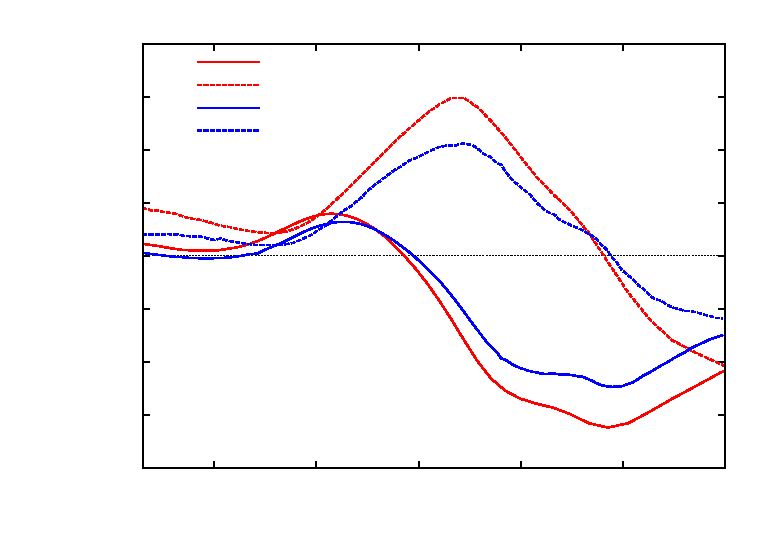
\includegraphics{PLD186t}}%
    \gplfronttext
  \end{picture}%
\endgroup

\caption{Spektrum polárního Kerrova jevu vzorku PLD186. Červené křivky odpovídají metodě zkřížených polarizátorl, modré pak teoretickým hodnotám.}
\label{sPLD186t}
\end{figure}

\begin{figure}
% GNUPLOT: LaTeX picture with Postscript
\begingroup
  \makeatletter
  \providecommand\color[2][]{%
    \GenericError{(gnuplot) \space\space\space\@spaces}{%
      Package color not loaded in conjunction with
      terminal option `colourtext'%
    }{See the gnuplot documentation for explanation.%
    }{Either use 'blacktext' in gnuplot or load the package
      color.sty in LaTeX.}%
    \renewcommand\color[2][]{}%
  }%
  \providecommand\includegraphics[2][]{%
    \GenericError{(gnuplot) \space\space\space\@spaces}{%
      Package graphicx or graphics not loaded%
    }{See the gnuplot documentation for explanation.%
    }{The gnuplot epslatex terminal needs graphicx.sty or graphics.sty.}%
    \renewcommand\includegraphics[2][]{}%
  }%
  \providecommand\rotatebox[2]{#2}%
  \@ifundefined{ifGPcolor}{%
    \newif\ifGPcolor
    \GPcolortrue
  }{}%
  \@ifundefined{ifGPblacktext}{%
    \newif\ifGPblacktext
    \GPblacktexttrue
  }{}%
  % define a \g@addto@macro without @ in the name:
  \let\gplgaddtomacro\g@addto@macro
  % define empty templates for all commands taking text:
  \gdef\gplbacktext{}%
  \gdef\gplfronttext{}%
  \makeatother
  \ifGPblacktext
    % no textcolor at all
    \def\colorrgb#1{}%
    \def\colorgray#1{}%
  \else
    % gray or color?
    \ifGPcolor
      \def\colorrgb#1{\color[rgb]{#1}}%
      \def\colorgray#1{\color[gray]{#1}}%
      \expandafter\def\csname LTw\endcsname{\color{white}}%
      \expandafter\def\csname LTb\endcsname{\color{black}}%
      \expandafter\def\csname LTa\endcsname{\color{black}}%
      \expandafter\def\csname LT0\endcsname{\color[rgb]{1,0,0}}%
      \expandafter\def\csname LT1\endcsname{\color[rgb]{0,1,0}}%
      \expandafter\def\csname LT2\endcsname{\color[rgb]{0,0,1}}%
      \expandafter\def\csname LT3\endcsname{\color[rgb]{1,0,1}}%
      \expandafter\def\csname LT4\endcsname{\color[rgb]{0,1,1}}%
      \expandafter\def\csname LT5\endcsname{\color[rgb]{1,1,0}}%
      \expandafter\def\csname LT6\endcsname{\color[rgb]{0,0,0}}%
      \expandafter\def\csname LT7\endcsname{\color[rgb]{1,0.3,0}}%
      \expandafter\def\csname LT8\endcsname{\color[rgb]{0.5,0.5,0.5}}%
    \else
      % gray
      \def\colorrgb#1{\color{black}}%
      \def\colorgray#1{\color[gray]{#1}}%
      \expandafter\def\csname LTw\endcsname{\color{white}}%
      \expandafter\def\csname LTb\endcsname{\color{black}}%
      \expandafter\def\csname LTa\endcsname{\color{black}}%
      \expandafter\def\csname LT0\endcsname{\color{black}}%
      \expandafter\def\csname LT1\endcsname{\color{black}}%
      \expandafter\def\csname LT2\endcsname{\color{black}}%
      \expandafter\def\csname LT3\endcsname{\color{black}}%
      \expandafter\def\csname LT4\endcsname{\color{black}}%
      \expandafter\def\csname LT5\endcsname{\color{black}}%
      \expandafter\def\csname LT6\endcsname{\color{black}}%
      \expandafter\def\csname LT7\endcsname{\color{black}}%
      \expandafter\def\csname LT8\endcsname{\color{black}}%
    \fi
  \fi
  \setlength{\unitlength}{0.0500bp}%
  \begin{picture}(7200.00,5040.00)%
    \gplgaddtomacro\gplbacktext{%
      \csname LTb\endcsname%
      \put(1078,704){\makebox(0,0)[r]{\strut{}-0.25}}%
      \put(1078,1156){\makebox(0,0)[r]{\strut{}-0.2}}%
      \put(1078,1609){\makebox(0,0)[r]{\strut{}-0.15}}%
      \put(1078,2061){\makebox(0,0)[r]{\strut{}-0.1}}%
      \put(1078,2513){\makebox(0,0)[r]{\strut{}-0.05}}%
      \put(1078,2966){\makebox(0,0)[r]{\strut{} 0}}%
      \put(1078,3418){\makebox(0,0)[r]{\strut{} 0.05}}%
      \put(1078,3870){\makebox(0,0)[r]{\strut{} 0.1}}%
      \put(1078,4323){\makebox(0,0)[r]{\strut{} 0.15}}%
      \put(1078,4775){\makebox(0,0)[r]{\strut{} 0.2}}%
      \put(1897,484){\makebox(0,0){\strut{} 2}}%
      \put(2878,484){\makebox(0,0){\strut{} 2.5}}%
      \put(3859,484){\makebox(0,0){\strut{} 3}}%
      \put(4841,484){\makebox(0,0){\strut{} 3.5}}%
      \put(5822,484){\makebox(0,0){\strut{} 4}}%
      \put(6803,484){\makebox(0,0){\strut{} 4.5}}%
      \csname LTb\endcsname%
      \put(176,2739){\rotatebox{-270}{\makebox(0,0){\strut{}Polární Kerrův jev [deg.]}}}%
      \put(4006,154){\makebox(0,0){\strut{}$E$ [eV]}}%
    }%
    \gplgaddtomacro\gplfronttext{%
      \csname LTb\endcsname%
      \put(1606,1537){\makebox(0,0)[r]{\strut{}$\theta_K$}}%
      \csname LTb\endcsname%
      \put(1606,1317){\makebox(0,0)[r]{\strut{}$\epsilon_K$}}%
      \csname LTb\endcsname%
      \put(1606,1097){\makebox(0,0)[r]{\strut{}$\theta_K$}}%
      \csname LTb\endcsname%
      \put(1606,877){\makebox(0,0)[r]{\strut{}$\epsilon_K$}}%
    }%
    \gplbacktext
    \put(0,0){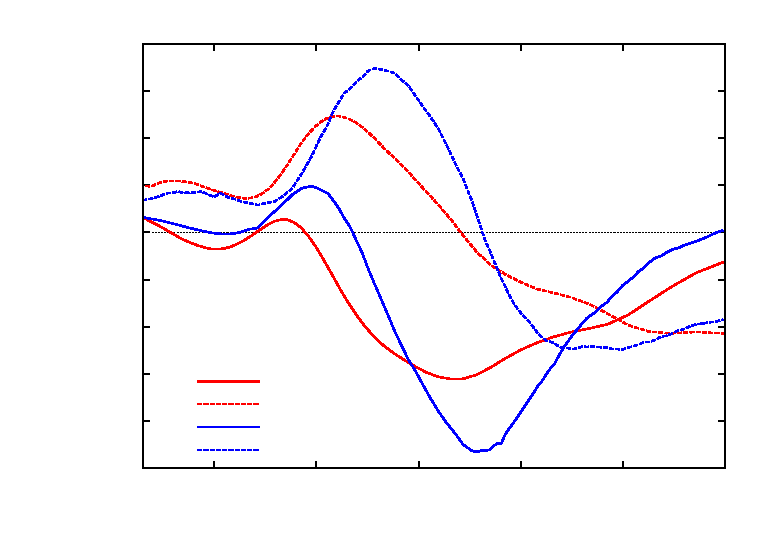
\includegraphics{PLD202t}}%
    \gplfronttext
  \end{picture}%
\endgroup

\caption{Spektrum polárního Kerrova jevu vzorku PLD202. Červené křivky odpovídají metodě zkřížených polarizátorl, modré pak teoretickým hodnotám.}
\label{sPLD202t}
\end{figure}
\section{Kobaltové feritové tenké vrstvy}
Další velmi intenzivně studovanou skupinou materiálů jsou oxidy železa.
Tyto materiály mají dobrý potenciál pro použití v mikrovlnných zařízeních a  pro magnetooptický zápis. 
Jejich hlavní předností je vysoká Curiova teplota, vysoká koercitiva a velká magnetická anizotropie. 

Tenké vrstvy kobaltového feritu (CoFe$_2$O$_4$) jsou obzvláště zajímavé díky vysoké hustotě magnetického zápisu.
Naše vzorky byli připravené metodou PLD na substrát z amorfního taveného křemene. K odpaření terčíku byly použity 5 ns dlouhé pulsy Nd:YAG laseru. 
Deponování námi zkoumaných vzorků probáhala za pokojové teploty, následně byly vzorky zahřáty na 750 (CoF-RT-A750) resp. 1100 (CoF-RT-A1100) 
stupňů Celsia. Tato teplota byla udržována po dobu dvou hodin, po kterých se vzorky nechaly schladit opět na pokojovou teplotu. Tloušťka vrstev je 110 nm.

Změřená spektra koblatových feritů jsou zobrazeny na obrázcích (\ref{sCoF-RT-A750}) a (\ref{sCoF-RT-A1100}). Z nich je dobře vidět, že vzorek je až do přibližně 2.7 eV značně transparentní, protože na spektru vznikl interferenčí obrazec pro tenkou vrstvu. Výsledky metod se v této oblasti liší, protože úhel dopadu se u metod odlišuje, což má za následek zdánlivý rozdíl 
v tloušťce vzorku. 

Nad 2.5 eV je spektrum už typické pro ferity. Konkrétně má velmi podobné spektrum jako lithný nebo mědnatý ferit. %\cite{ferity} 

Dále je vidět vliv teploty, při které byly vzorky deponovány, na spektrum vzorku. Při vysokých teplotách totiž zřejmě dochází k materiálovým změnám, které mají za následek pokles magnetizace ve vzorku, a tím pádem i magnetooptické odezvy.


\begin{figure}
% GNUPLOT: LaTeX picture with Postscript
\begingroup
  \makeatletter
  \providecommand\color[2][]{%
    \GenericError{(gnuplot) \space\space\space\@spaces}{%
      Package color not loaded in conjunction with
      terminal option `colourtext'%
    }{See the gnuplot documentation for explanation.%
    }{Either use 'blacktext' in gnuplot or load the package
      color.sty in LaTeX.}%
    \renewcommand\color[2][]{}%
  }%
  \providecommand\includegraphics[2][]{%
    \GenericError{(gnuplot) \space\space\space\@spaces}{%
      Package graphicx or graphics not loaded%
    }{See the gnuplot documentation for explanation.%
    }{The gnuplot epslatex terminal needs graphicx.sty or graphics.sty.}%
    \renewcommand\includegraphics[2][]{}%
  }%
  \providecommand\rotatebox[2]{#2}%
  \@ifundefined{ifGPcolor}{%
    \newif\ifGPcolor
    \GPcolortrue
  }{}%
  \@ifundefined{ifGPblacktext}{%
    \newif\ifGPblacktext
    \GPblacktexttrue
  }{}%
  % define a \g@addto@macro without @ in the name:
  \let\gplgaddtomacro\g@addto@macro
  % define empty templates for all commands taking text:
  \gdef\gplbacktext{}%
  \gdef\gplfronttext{}%
  \makeatother
  \ifGPblacktext
    % no textcolor at all
    \def\colorrgb#1{}%
    \def\colorgray#1{}%
  \else
    % gray or color?
    \ifGPcolor
      \def\colorrgb#1{\color[rgb]{#1}}%
      \def\colorgray#1{\color[gray]{#1}}%
      \expandafter\def\csname LTw\endcsname{\color{white}}%
      \expandafter\def\csname LTb\endcsname{\color{black}}%
      \expandafter\def\csname LTa\endcsname{\color{black}}%
      \expandafter\def\csname LT0\endcsname{\color[rgb]{1,0,0}}%
      \expandafter\def\csname LT1\endcsname{\color[rgb]{0,1,0}}%
      \expandafter\def\csname LT2\endcsname{\color[rgb]{0,0,1}}%
      \expandafter\def\csname LT3\endcsname{\color[rgb]{1,0,1}}%
      \expandafter\def\csname LT4\endcsname{\color[rgb]{0,1,1}}%
      \expandafter\def\csname LT5\endcsname{\color[rgb]{1,1,0}}%
      \expandafter\def\csname LT6\endcsname{\color[rgb]{0,0,0}}%
      \expandafter\def\csname LT7\endcsname{\color[rgb]{1,0.3,0}}%
      \expandafter\def\csname LT8\endcsname{\color[rgb]{0.5,0.5,0.5}}%
    \else
      % gray
      \def\colorrgb#1{\color{black}}%
      \def\colorgray#1{\color[gray]{#1}}%
      \expandafter\def\csname LTw\endcsname{\color{white}}%
      \expandafter\def\csname LTb\endcsname{\color{black}}%
      \expandafter\def\csname LTa\endcsname{\color{black}}%
      \expandafter\def\csname LT0\endcsname{\color{black}}%
      \expandafter\def\csname LT1\endcsname{\color{black}}%
      \expandafter\def\csname LT2\endcsname{\color{black}}%
      \expandafter\def\csname LT3\endcsname{\color{black}}%
      \expandafter\def\csname LT4\endcsname{\color{black}}%
      \expandafter\def\csname LT5\endcsname{\color{black}}%
      \expandafter\def\csname LT6\endcsname{\color{black}}%
      \expandafter\def\csname LT7\endcsname{\color{black}}%
      \expandafter\def\csname LT8\endcsname{\color{black}}%
    \fi
  \fi
  \setlength{\unitlength}{0.0500bp}%
  \begin{picture}(7200.00,5040.00)%
    \gplgaddtomacro\gplbacktext{%
      \csname LTb\endcsname%
      \put(946,704){\makebox(0,0)[r]{\strut{}-0.6}}%
      \put(946,1383){\makebox(0,0)[r]{\strut{}-0.4}}%
      \put(946,2061){\makebox(0,0)[r]{\strut{}-0.2}}%
      \put(946,2740){\makebox(0,0)[r]{\strut{} 0}}%
      \put(946,3418){\makebox(0,0)[r]{\strut{} 0.2}}%
      \put(946,4097){\makebox(0,0)[r]{\strut{} 0.4}}%
      \put(946,4775){\makebox(0,0)[r]{\strut{} 0.6}}%
      \put(1257,484){\makebox(0,0){\strut{} 1.5}}%
      \put(2151,484){\makebox(0,0){\strut{} 2}}%
      \put(3046,484){\makebox(0,0){\strut{} 2.5}}%
      \put(3941,484){\makebox(0,0){\strut{} 3}}%
      \put(4835,484){\makebox(0,0){\strut{} 3.5}}%
      \put(5730,484){\makebox(0,0){\strut{} 4}}%
      \put(6624,484){\makebox(0,0){\strut{} 4.5}}%
      \csname LTb\endcsname%
      \put(176,2739){\rotatebox{-270}{\makebox(0,0){\strut{}Polární Kerrův jev [deg.]}}}%
      \put(3940,154){\makebox(0,0){\strut{}$E$ [eV]}}%
    }%
    \gplgaddtomacro\gplfronttext{%
      \csname LTb\endcsname%
      \put(5816,4602){\makebox(0,0)[r]{\strut{}$\theta_K$}}%
      \csname LTb\endcsname%
      \put(5816,4382){\makebox(0,0)[r]{\strut{}$\epsilon_K$}}%
      \csname LTb\endcsname%
      \put(5816,4162){\makebox(0,0)[r]{\strut{}$\theta_K$}}%
      \csname LTb\endcsname%
      \put(5816,3942){\makebox(0,0)[r]{\strut{}$\epsilon_K$}}%
    }%
    \gplbacktext
    \put(0,0){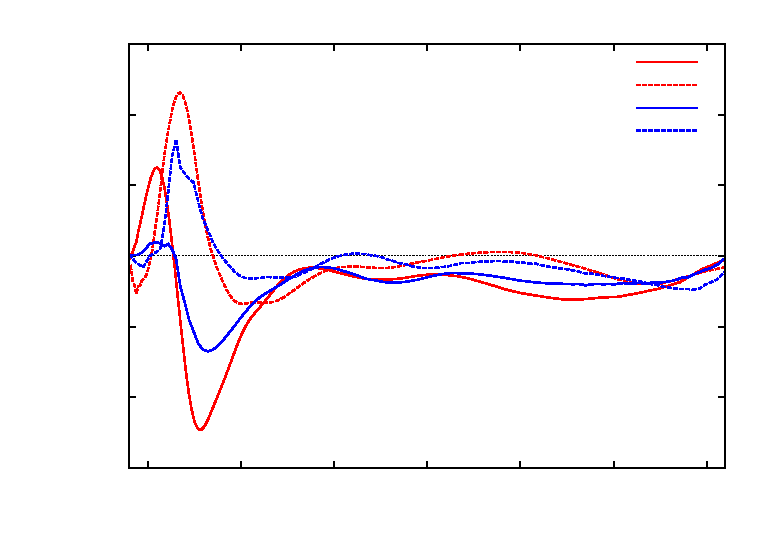
\includegraphics{CoF-RT-A750}}%
    \gplfronttext
  \end{picture}%
\endgroup

\caption{Spektrum polárního Kerrova jevu vzorku CoF-RT-A750. Červené křivky odpovídají metodě zkřížených polarizátorl, modré pak modulační metodě.}
\label{sCoF-RT-A750}
\end{figure}

\begin{figure}
% GNUPLOT: LaTeX picture with Postscript
\begingroup
  \makeatletter
  \providecommand\color[2][]{%
    \GenericError{(gnuplot) \space\space\space\@spaces}{%
      Package color not loaded in conjunction with
      terminal option `colourtext'%
    }{See the gnuplot documentation for explanation.%
    }{Either use 'blacktext' in gnuplot or load the package
      color.sty in LaTeX.}%
    \renewcommand\color[2][]{}%
  }%
  \providecommand\includegraphics[2][]{%
    \GenericError{(gnuplot) \space\space\space\@spaces}{%
      Package graphicx or graphics not loaded%
    }{See the gnuplot documentation for explanation.%
    }{The gnuplot epslatex terminal needs graphicx.sty or graphics.sty.}%
    \renewcommand\includegraphics[2][]{}%
  }%
  \providecommand\rotatebox[2]{#2}%
  \@ifundefined{ifGPcolor}{%
    \newif\ifGPcolor
    \GPcolorfalse
  }{}%
  \@ifundefined{ifGPblacktext}{%
    \newif\ifGPblacktext
    \GPblacktexttrue
  }{}%
  % define a \g@addto@macro without @ in the name:
  \let\gplgaddtomacro\g@addto@macro
  % define empty templates for all commands taking text:
  \gdef\gplbacktext{}%
  \gdef\gplfronttext{}%
  \makeatother
  \ifGPblacktext
    % no textcolor at all
    \def\colorrgb#1{}%
    \def\colorgray#1{}%
  \else
    % gray or color?
    \ifGPcolor
      \def\colorrgb#1{\color[rgb]{#1}}%
      \def\colorgray#1{\color[gray]{#1}}%
      \expandafter\def\csname LTw\endcsname{\color{white}}%
      \expandafter\def\csname LTb\endcsname{\color{black}}%
      \expandafter\def\csname LTa\endcsname{\color{black}}%
      \expandafter\def\csname LT0\endcsname{\color[rgb]{1,0,0}}%
      \expandafter\def\csname LT1\endcsname{\color[rgb]{0,1,0}}%
      \expandafter\def\csname LT2\endcsname{\color[rgb]{0,0,1}}%
      \expandafter\def\csname LT3\endcsname{\color[rgb]{1,0,1}}%
      \expandafter\def\csname LT4\endcsname{\color[rgb]{0,1,1}}%
      \expandafter\def\csname LT5\endcsname{\color[rgb]{1,1,0}}%
      \expandafter\def\csname LT6\endcsname{\color[rgb]{0,0,0}}%
      \expandafter\def\csname LT7\endcsname{\color[rgb]{1,0.3,0}}%
      \expandafter\def\csname LT8\endcsname{\color[rgb]{0.5,0.5,0.5}}%
    \else
      % gray
      \def\colorrgb#1{\color{black}}%
      \def\colorgray#1{\color[gray]{#1}}%
      \expandafter\def\csname LTw\endcsname{\color{white}}%
      \expandafter\def\csname LTb\endcsname{\color{black}}%
      \expandafter\def\csname LTa\endcsname{\color{black}}%
      \expandafter\def\csname LT0\endcsname{\color{black}}%
      \expandafter\def\csname LT1\endcsname{\color{black}}%
      \expandafter\def\csname LT2\endcsname{\color{black}}%
      \expandafter\def\csname LT3\endcsname{\color{black}}%
      \expandafter\def\csname LT4\endcsname{\color{black}}%
      \expandafter\def\csname LT5\endcsname{\color{black}}%
      \expandafter\def\csname LT6\endcsname{\color{black}}%
      \expandafter\def\csname LT7\endcsname{\color{black}}%
      \expandafter\def\csname LT8\endcsname{\color{black}}%
    \fi
  \fi
  \setlength{\unitlength}{0.0500bp}%
  \begin{picture}(7200.00,5040.00)%
    \gplgaddtomacro\gplbacktext{%
      \csname LTb\endcsname%
      \put(1078,704){\makebox(0,0)[r]{\strut{}-0.4}}%
      \put(1078,1213){\makebox(0,0)[r]{\strut{}-0.3}}%
      \put(1078,1722){\makebox(0,0)[r]{\strut{}-0.2}}%
      \put(1078,2231){\makebox(0,0)[r]{\strut{}-0.1}}%
      \put(1078,2739){\makebox(0,0)[r]{\strut{} 0}}%
      \put(1078,3248){\makebox(0,0)[r]{\strut{} 0.1}}%
      \put(1078,3757){\makebox(0,0)[r]{\strut{} 0.2}}%
      \put(1078,4266){\makebox(0,0)[r]{\strut{} 0.3}}%
      \put(1078,4775){\makebox(0,0)[r]{\strut{} 0.4}}%
      \put(1367,484){\makebox(0,0){\strut{} 1.5}}%
      \put(2153,484){\makebox(0,0){\strut{} 2}}%
      \put(2939,484){\makebox(0,0){\strut{} 2.5}}%
      \put(3725,484){\makebox(0,0){\strut{} 3}}%
      \put(4511,484){\makebox(0,0){\strut{} 3.5}}%
      \put(5297,484){\makebox(0,0){\strut{} 4}}%
      \put(6083,484){\makebox(0,0){\strut{} 4.5}}%
      \put(6869,484){\makebox(0,0){\strut{} 5}}%
      \put(308,2739){\rotatebox{-270}{\makebox(0,0){\strut{}Polární Kerrův jev [deg.]}}}%
      \put(4039,154){\makebox(0,0){\strut{}$E$/eV}}%
    }%
    \gplgaddtomacro\gplfronttext{%
      \csname LTb\endcsname%
      \put(5882,4602){\makebox(0,0)[r]{\strut{}$\theta^1_K$}}%
      \csname LTb\endcsname%
      \put(5882,4382){\makebox(0,0)[r]{\strut{}$\epsilon^1_K$}}%
      \csname LTb\endcsname%
      \put(5882,4162){\makebox(0,0)[r]{\strut{}$\theta^2_K$}}%
      \csname LTb\endcsname%
      \put(5882,3942){\makebox(0,0)[r]{\strut{}$\epsilon^2_K$}}%
    }%
    \gplbacktext
    \put(0,0){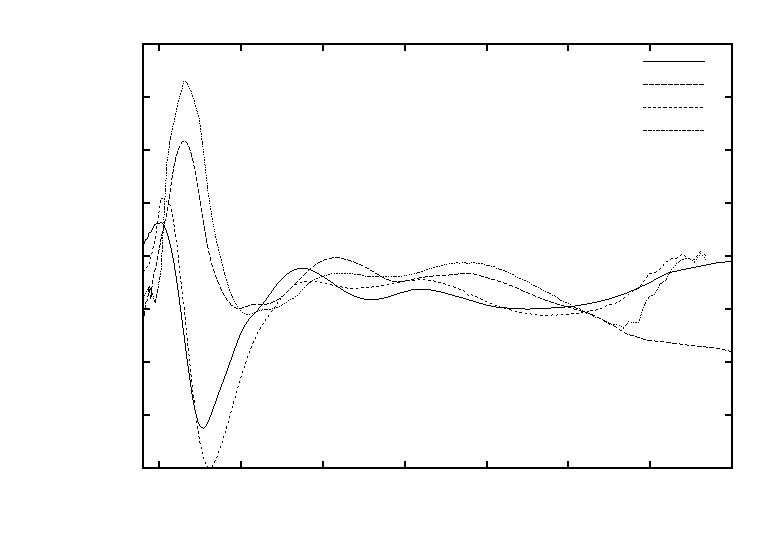
\includegraphics{grafy/CoF-RT-A1100}}%
    \gplfronttext
  \end{picture}%
\endgroup

\caption{Spektrum polárního Kerrova jevu vzorku CoF-RT-A1100. Červené křivky odpovídají metodě zkřížených polarizátorl, modré pak modulační metodě.}
\label{sCoF-RT-A1100}
\end{figure}

\section{Heuslerovy slitiny}
Jako poslední typ vzorků jsme použily zástupce z Heuslerovývh slitin. Tyto vzorky mají opět 
skvělé vlastnosti pro použití v oblasti spintroniky.  Námi zkoumané slitiny byly různou směsí kobaltu, 
železa a křemíku. Ze všech zástupců zkoumaných Heuslerových slitin mají tyto výrazně nejvyšší Curiovu 
teplotu ($\sim 1100$K). Pro srovnání se Curiova teplota Fe$_2$MnSi se pohybuje pod pokojovou teplotou.

Tyto materiály se vyrábí za pomoci nízkoteplotní molekulární svazkové epitaxie. Ve zkratce se při této 
metodě v oddělených komorách zahřívají jednotlivé koponenty. Jejich výpary vstupují do hlavní komory, ve které je velmi vysoké vakuum, kde následně kondenzují na substrátu. 
Rychlost růstu se pohybuje pod 3000 nm za hodinu, což umožňuje výrobu velmi tenkých filmů.

Deponování našich vzorků probíhalo na substrát MgO. Na něm byla deponována nejprve 5 nm tenká vrstva chrómu, následně 20 nm slitiny a navrchu 2 nm MgO. Poměry kovů ve slitinách byli 7:5 (CoFeSi1) a 2:1 (CoFeSi2) v prospěch kobaltu.

Spektra vzorků Heuslerových slitin jsou na obrázcích (\ref{sCoFeSi1}) a (\ref{sCoFeSi2}). Rozdílná velikost amplitud efektů je dána použitím různých magnetů. 
Magnet první z metod totiž nevytváří dostatečně velké pole pro nasycení vzorku. Porovnáním tvarů spekter však vidíme, že si výsledky obou metod odpovídají.

Ze spekter je také dobře vidět, že vetší přítomnost železa na úkor kobaltu má za následek větší efekt.

\begin{figure}
% GNUPLOT: LaTeX picture with Postscript
\begingroup
  \makeatletter
  \providecommand\color[2][]{%
    \GenericError{(gnuplot) \space\space\space\@spaces}{%
      Package color not loaded in conjunction with
      terminal option `colourtext'%
    }{See the gnuplot documentation for explanation.%
    }{Either use 'blacktext' in gnuplot or load the package
      color.sty in LaTeX.}%
    \renewcommand\color[2][]{}%
  }%
  \providecommand\includegraphics[2][]{%
    \GenericError{(gnuplot) \space\space\space\@spaces}{%
      Package graphicx or graphics not loaded%
    }{See the gnuplot documentation for explanation.%
    }{The gnuplot epslatex terminal needs graphicx.sty or graphics.sty.}%
    \renewcommand\includegraphics[2][]{}%
  }%
  \providecommand\rotatebox[2]{#2}%
  \@ifundefined{ifGPcolor}{%
    \newif\ifGPcolor
    \GPcolorfalse
  }{}%
  \@ifundefined{ifGPblacktext}{%
    \newif\ifGPblacktext
    \GPblacktexttrue
  }{}%
  % define a \g@addto@macro without @ in the name:
  \let\gplgaddtomacro\g@addto@macro
  % define empty templates for all commands taking text:
  \gdef\gplbacktext{}%
  \gdef\gplfronttext{}%
  \makeatother
  \ifGPblacktext
    % no textcolor at all
    \def\colorrgb#1{}%
    \def\colorgray#1{}%
  \else
    % gray or color?
    \ifGPcolor
      \def\colorrgb#1{\color[rgb]{#1}}%
      \def\colorgray#1{\color[gray]{#1}}%
      \expandafter\def\csname LTw\endcsname{\color{white}}%
      \expandafter\def\csname LTb\endcsname{\color{black}}%
      \expandafter\def\csname LTa\endcsname{\color{black}}%
      \expandafter\def\csname LT0\endcsname{\color[rgb]{1,0,0}}%
      \expandafter\def\csname LT1\endcsname{\color[rgb]{0,1,0}}%
      \expandafter\def\csname LT2\endcsname{\color[rgb]{0,0,1}}%
      \expandafter\def\csname LT3\endcsname{\color[rgb]{1,0,1}}%
      \expandafter\def\csname LT4\endcsname{\color[rgb]{0,1,1}}%
      \expandafter\def\csname LT5\endcsname{\color[rgb]{1,1,0}}%
      \expandafter\def\csname LT6\endcsname{\color[rgb]{0,0,0}}%
      \expandafter\def\csname LT7\endcsname{\color[rgb]{1,0.3,0}}%
      \expandafter\def\csname LT8\endcsname{\color[rgb]{0.5,0.5,0.5}}%
    \else
      % gray
      \def\colorrgb#1{\color{black}}%
      \def\colorgray#1{\color[gray]{#1}}%
      \expandafter\def\csname LTw\endcsname{\color{white}}%
      \expandafter\def\csname LTb\endcsname{\color{black}}%
      \expandafter\def\csname LTa\endcsname{\color{black}}%
      \expandafter\def\csname LT0\endcsname{\color{black}}%
      \expandafter\def\csname LT1\endcsname{\color{black}}%
      \expandafter\def\csname LT2\endcsname{\color{black}}%
      \expandafter\def\csname LT3\endcsname{\color{black}}%
      \expandafter\def\csname LT4\endcsname{\color{black}}%
      \expandafter\def\csname LT5\endcsname{\color{black}}%
      \expandafter\def\csname LT6\endcsname{\color{black}}%
      \expandafter\def\csname LT7\endcsname{\color{black}}%
      \expandafter\def\csname LT8\endcsname{\color{black}}%
    \fi
  \fi
  \setlength{\unitlength}{0.0500bp}%
  \begin{picture}(7200.00,5040.00)%
    \gplgaddtomacro\gplbacktext{%
      \csname LTb\endcsname%
      \put(1122,704){\makebox(0,0)[r]{\strut{}-0.008}}%
      \put(1122,1213){\makebox(0,0)[r]{\strut{}-0.006}}%
      \put(1122,1722){\makebox(0,0)[r]{\strut{}-0.004}}%
      \put(1122,2231){\makebox(0,0)[r]{\strut{}-0.002}}%
      \put(1122,2740){\makebox(0,0)[r]{\strut{} 0}}%
      \put(1122,3248){\makebox(0,0)[r]{\strut{} 0.002}}%
      \put(1122,3757){\makebox(0,0)[r]{\strut{} 0.004}}%
      \put(1122,4266){\makebox(0,0)[r]{\strut{} 0.006}}%
      \put(1122,4775){\makebox(0,0)[r]{\strut{} 0.008}}%
      \put(1410,484){\makebox(0,0){\strut{} 1.5}}%
      \put(2190,484){\makebox(0,0){\strut{} 2}}%
      \put(2970,484){\makebox(0,0){\strut{} 2.5}}%
      \put(3750,484){\makebox(0,0){\strut{} 3}}%
      \put(4529,484){\makebox(0,0){\strut{} 3.5}}%
      \put(5309,484){\makebox(0,0){\strut{} 4}}%
      \put(6089,484){\makebox(0,0){\strut{} 4.5}}%
      \put(6869,484){\makebox(0,0){\strut{} 5}}%
      \put(308,2739){\rotatebox{-270}{\makebox(0,0){\strut{}}}}%
      \put(4061,154){\makebox(0,0){\strut{}$E$/eV}}%
    }%
    \gplgaddtomacro\gplfronttext{%
      \csname LTb\endcsname%
      \put(2970,4602){\makebox(0,0)[r]{\strut{}$\theta_K$}}%
      \csname LTb\endcsname%
      \put(2970,4382){\makebox(0,0)[r]{\strut{}$\epsilon_K$}}%
    }%
    \gplbacktext
    \put(0,0){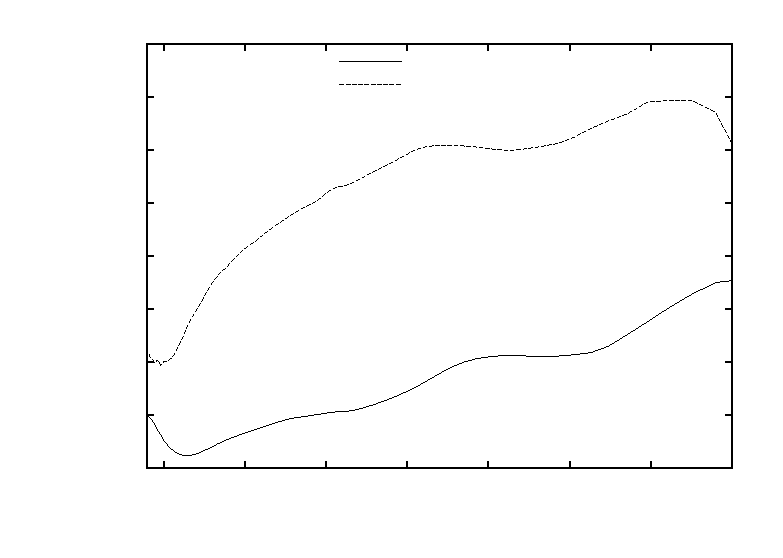
\includegraphics{CoFeSi1}}%
    \gplfronttext
  \end{picture}%
\endgroup

\caption{Spektrum polárního Kerrova jevu vzorku CoFeSi1. Červené křivky odpovídají metodě zkřížených polarizátorl, modré pak modulační metodě.}
\label{sCoFeSi1}
\end{figure}

\begin{figure}
% GNUPLOT: LaTeX picture with Postscript
\begingroup
  \makeatletter
  \providecommand\color[2][]{%
    \GenericError{(gnuplot) \space\space\space\@spaces}{%
      Package color not loaded in conjunction with
      terminal option `colourtext'%
    }{See the gnuplot documentation for explanation.%
    }{Either use 'blacktext' in gnuplot or load the package
      color.sty in LaTeX.}%
    \renewcommand\color[2][]{}%
  }%
  \providecommand\includegraphics[2][]{%
    \GenericError{(gnuplot) \space\space\space\@spaces}{%
      Package graphicx or graphics not loaded%
    }{See the gnuplot documentation for explanation.%
    }{The gnuplot epslatex terminal needs graphicx.sty or graphics.sty.}%
    \renewcommand\includegraphics[2][]{}%
  }%
  \providecommand\rotatebox[2]{#2}%
  \@ifundefined{ifGPcolor}{%
    \newif\ifGPcolor
    \GPcolortrue
  }{}%
  \@ifundefined{ifGPblacktext}{%
    \newif\ifGPblacktext
    \GPblacktexttrue
  }{}%
  % define a \g@addto@macro without @ in the name:
  \let\gplgaddtomacro\g@addto@macro
  % define empty templates for all commands taking text:
  \gdef\gplbacktext{}%
  \gdef\gplfronttext{}%
  \makeatother
  \ifGPblacktext
    % no textcolor at all
    \def\colorrgb#1{}%
    \def\colorgray#1{}%
  \else
    % gray or color?
    \ifGPcolor
      \def\colorrgb#1{\color[rgb]{#1}}%
      \def\colorgray#1{\color[gray]{#1}}%
      \expandafter\def\csname LTw\endcsname{\color{white}}%
      \expandafter\def\csname LTb\endcsname{\color{black}}%
      \expandafter\def\csname LTa\endcsname{\color{black}}%
      \expandafter\def\csname LT0\endcsname{\color[rgb]{1,0,0}}%
      \expandafter\def\csname LT1\endcsname{\color[rgb]{0,1,0}}%
      \expandafter\def\csname LT2\endcsname{\color[rgb]{0,0,1}}%
      \expandafter\def\csname LT3\endcsname{\color[rgb]{1,0,1}}%
      \expandafter\def\csname LT4\endcsname{\color[rgb]{0,1,1}}%
      \expandafter\def\csname LT5\endcsname{\color[rgb]{1,1,0}}%
      \expandafter\def\csname LT6\endcsname{\color[rgb]{0,0,0}}%
      \expandafter\def\csname LT7\endcsname{\color[rgb]{1,0.3,0}}%
      \expandafter\def\csname LT8\endcsname{\color[rgb]{0.5,0.5,0.5}}%
    \else
      % gray
      \def\colorrgb#1{\color{black}}%
      \def\colorgray#1{\color[gray]{#1}}%
      \expandafter\def\csname LTw\endcsname{\color{white}}%
      \expandafter\def\csname LTb\endcsname{\color{black}}%
      \expandafter\def\csname LTa\endcsname{\color{black}}%
      \expandafter\def\csname LT0\endcsname{\color{black}}%
      \expandafter\def\csname LT1\endcsname{\color{black}}%
      \expandafter\def\csname LT2\endcsname{\color{black}}%
      \expandafter\def\csname LT3\endcsname{\color{black}}%
      \expandafter\def\csname LT4\endcsname{\color{black}}%
      \expandafter\def\csname LT5\endcsname{\color{black}}%
      \expandafter\def\csname LT6\endcsname{\color{black}}%
      \expandafter\def\csname LT7\endcsname{\color{black}}%
      \expandafter\def\csname LT8\endcsname{\color{black}}%
    \fi
  \fi
  \setlength{\unitlength}{0.0500bp}%
  \begin{picture}(7200.00,5040.00)%
    \gplgaddtomacro\gplbacktext{%
      \csname LTb\endcsname%
      \put(1078,704){\makebox(0,0)[r]{\strut{}-0.3}}%
      \put(1078,1156){\makebox(0,0)[r]{\strut{}-0.25}}%
      \put(1078,1609){\makebox(0,0)[r]{\strut{}-0.2}}%
      \put(1078,2061){\makebox(0,0)[r]{\strut{}-0.15}}%
      \put(1078,2513){\makebox(0,0)[r]{\strut{}-0.1}}%
      \put(1078,2966){\makebox(0,0)[r]{\strut{}-0.05}}%
      \put(1078,3418){\makebox(0,0)[r]{\strut{} 0}}%
      \put(1078,3870){\makebox(0,0)[r]{\strut{} 0.05}}%
      \put(1078,4323){\makebox(0,0)[r]{\strut{} 0.1}}%
      \put(1078,4775){\makebox(0,0)[r]{\strut{} 0.15}}%
      \put(1379,484){\makebox(0,0){\strut{} 1.5}}%
      \put(2227,484){\makebox(0,0){\strut{} 2}}%
      \put(3074,484){\makebox(0,0){\strut{} 2.5}}%
      \put(3922,484){\makebox(0,0){\strut{} 3}}%
      \put(4769,484){\makebox(0,0){\strut{} 3.5}}%
      \put(5617,484){\makebox(0,0){\strut{} 4}}%
      \put(6464,484){\makebox(0,0){\strut{} 4.5}}%
      \csname LTb\endcsname%
      \put(176,2739){\rotatebox{-270}{\makebox(0,0){\strut{}Polární Kerrův jev [deg.]}}}%
      \put(4006,154){\makebox(0,0){\strut{}$E$ [eV]}}%
    }%
    \gplgaddtomacro\gplfronttext{%
      \csname LTb\endcsname%
      \put(5816,1537){\makebox(0,0)[r]{\strut{}$\theta_K$}}%
      \csname LTb\endcsname%
      \put(5816,1317){\makebox(0,0)[r]{\strut{}$\epsilon_K$}}%
      \csname LTb\endcsname%
      \put(5816,1097){\makebox(0,0)[r]{\strut{}$\theta_K$}}%
      \csname LTb\endcsname%
      \put(5816,877){\makebox(0,0)[r]{\strut{}$\epsilon_K$}}%
    }%
    \gplbacktext
    \put(0,0){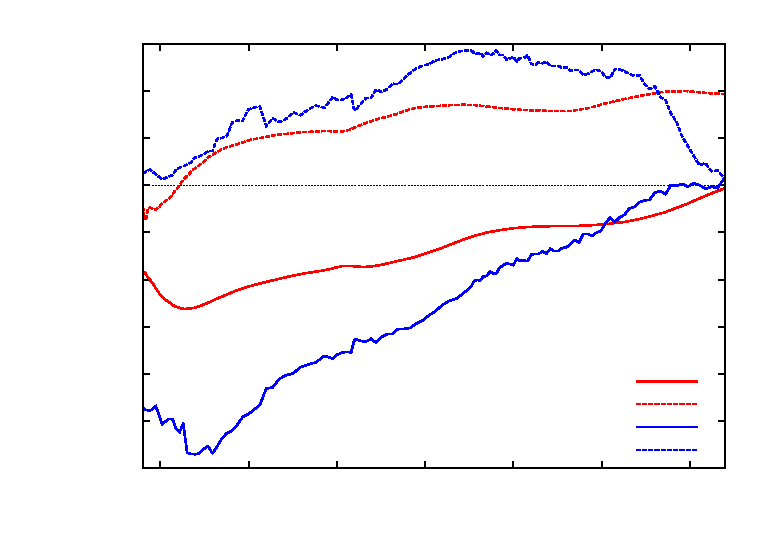
\includegraphics{CoFeSi2}}%
    \gplfronttext
  \end{picture}%
\endgroup

\caption{Spektrum polárního Kerrova jevu vzorku CoFeSi2. Červené křivky odpovídají metodě zkřížených polarizátorl, modré pak modulační metodě.}
\label{sCoFeSi2}
\end{figure}
